\documentclass[a4paper,12pt]{article}
%\usepackage{fullpage}
%\usepackage{pdfpages}

\usepackage{geometry}
 \geometry{
 a4paper,
 total={170mm,257mm},
 left=20mm,
 top=20mm,
 }

\usepackage{color}
\usepackage{amsmath,graphicx,makeidx}
\usepackage{lscape}
\usepackage{fancyhdr}
\addtolength{\headheight}{1.5cm} % make more space for the header
\pagestyle{fancyplain} % use fancy for all pages except chapter start
\lhead{
\includegraphics[height=1.7cm]{FOSSEE-logo}} % left logo
\rhead{
\includegraphics[height=3.5cm]{DWSIM-flowsheeting-project-logo}} % right logo
\renewcommand{\headrulewidth}{0pt} % remove rule below header

\title{Sour Water Stripping}
\author{Daniel Wagner \\ DWSIM Developer}
\date{}

\begin{document}

\maketitle

\noindent \textbf{Background \& Description:}
\newline Sour Water is the wastewater that is produced from atmospheric and vacuum crude columns at refineries. Hydrogen sulfide ($H_2S$) and ammonia ($NH_3$) are typical components in sour water that need to be removed before the water can be reused elsewhere in the plant. Removal of these components is done by sending the sour water from the process to a stripping tower where heat, in the form of steam, is applied. The ammonia and hydrogen sulfide contained in the water is released by the heat and exits the top of the tower.
The gases removed from sour water received from the refinery are known as sour Gas and are pumped off to the Sulfur Recovery Unit (SRU). This degassed sour water is pumped into a storage tank that serves to dampen the flow rate and facilitates removal of entrained oil and solids.


The first step in this process is known as hydrogen sulfide stripping. The degassed sour water is fed to the acid gas or $H_2S$ stripper column, which is a steam-reboiled distillation column. The hydrogen sulfide, which is stripped overhead, is of high purity - an excellent feed for sulfur recovery units or sulfuric acid plants. The column used for the purpose of $H_2S$ stripping has 20 stages and is operated with reflux ratio of 2.


Next, the hydrogen sulfide stripper stream, containing all the ammonia in the feed water and some hydrogen sulfide, is fed directly to the $NH_3$ stripper column, which is a refluxed distillation column. In this column, essentially all ammonia and hydrogen sulfide are removed from the water. This column has 12 stages with feed entering at 2nd stage. After exchanging heat with the hydrogen sulfide stripper feed, the stripped water is cooled and sent off for either reuse or treating.


\vspace{10mm}
\centerline{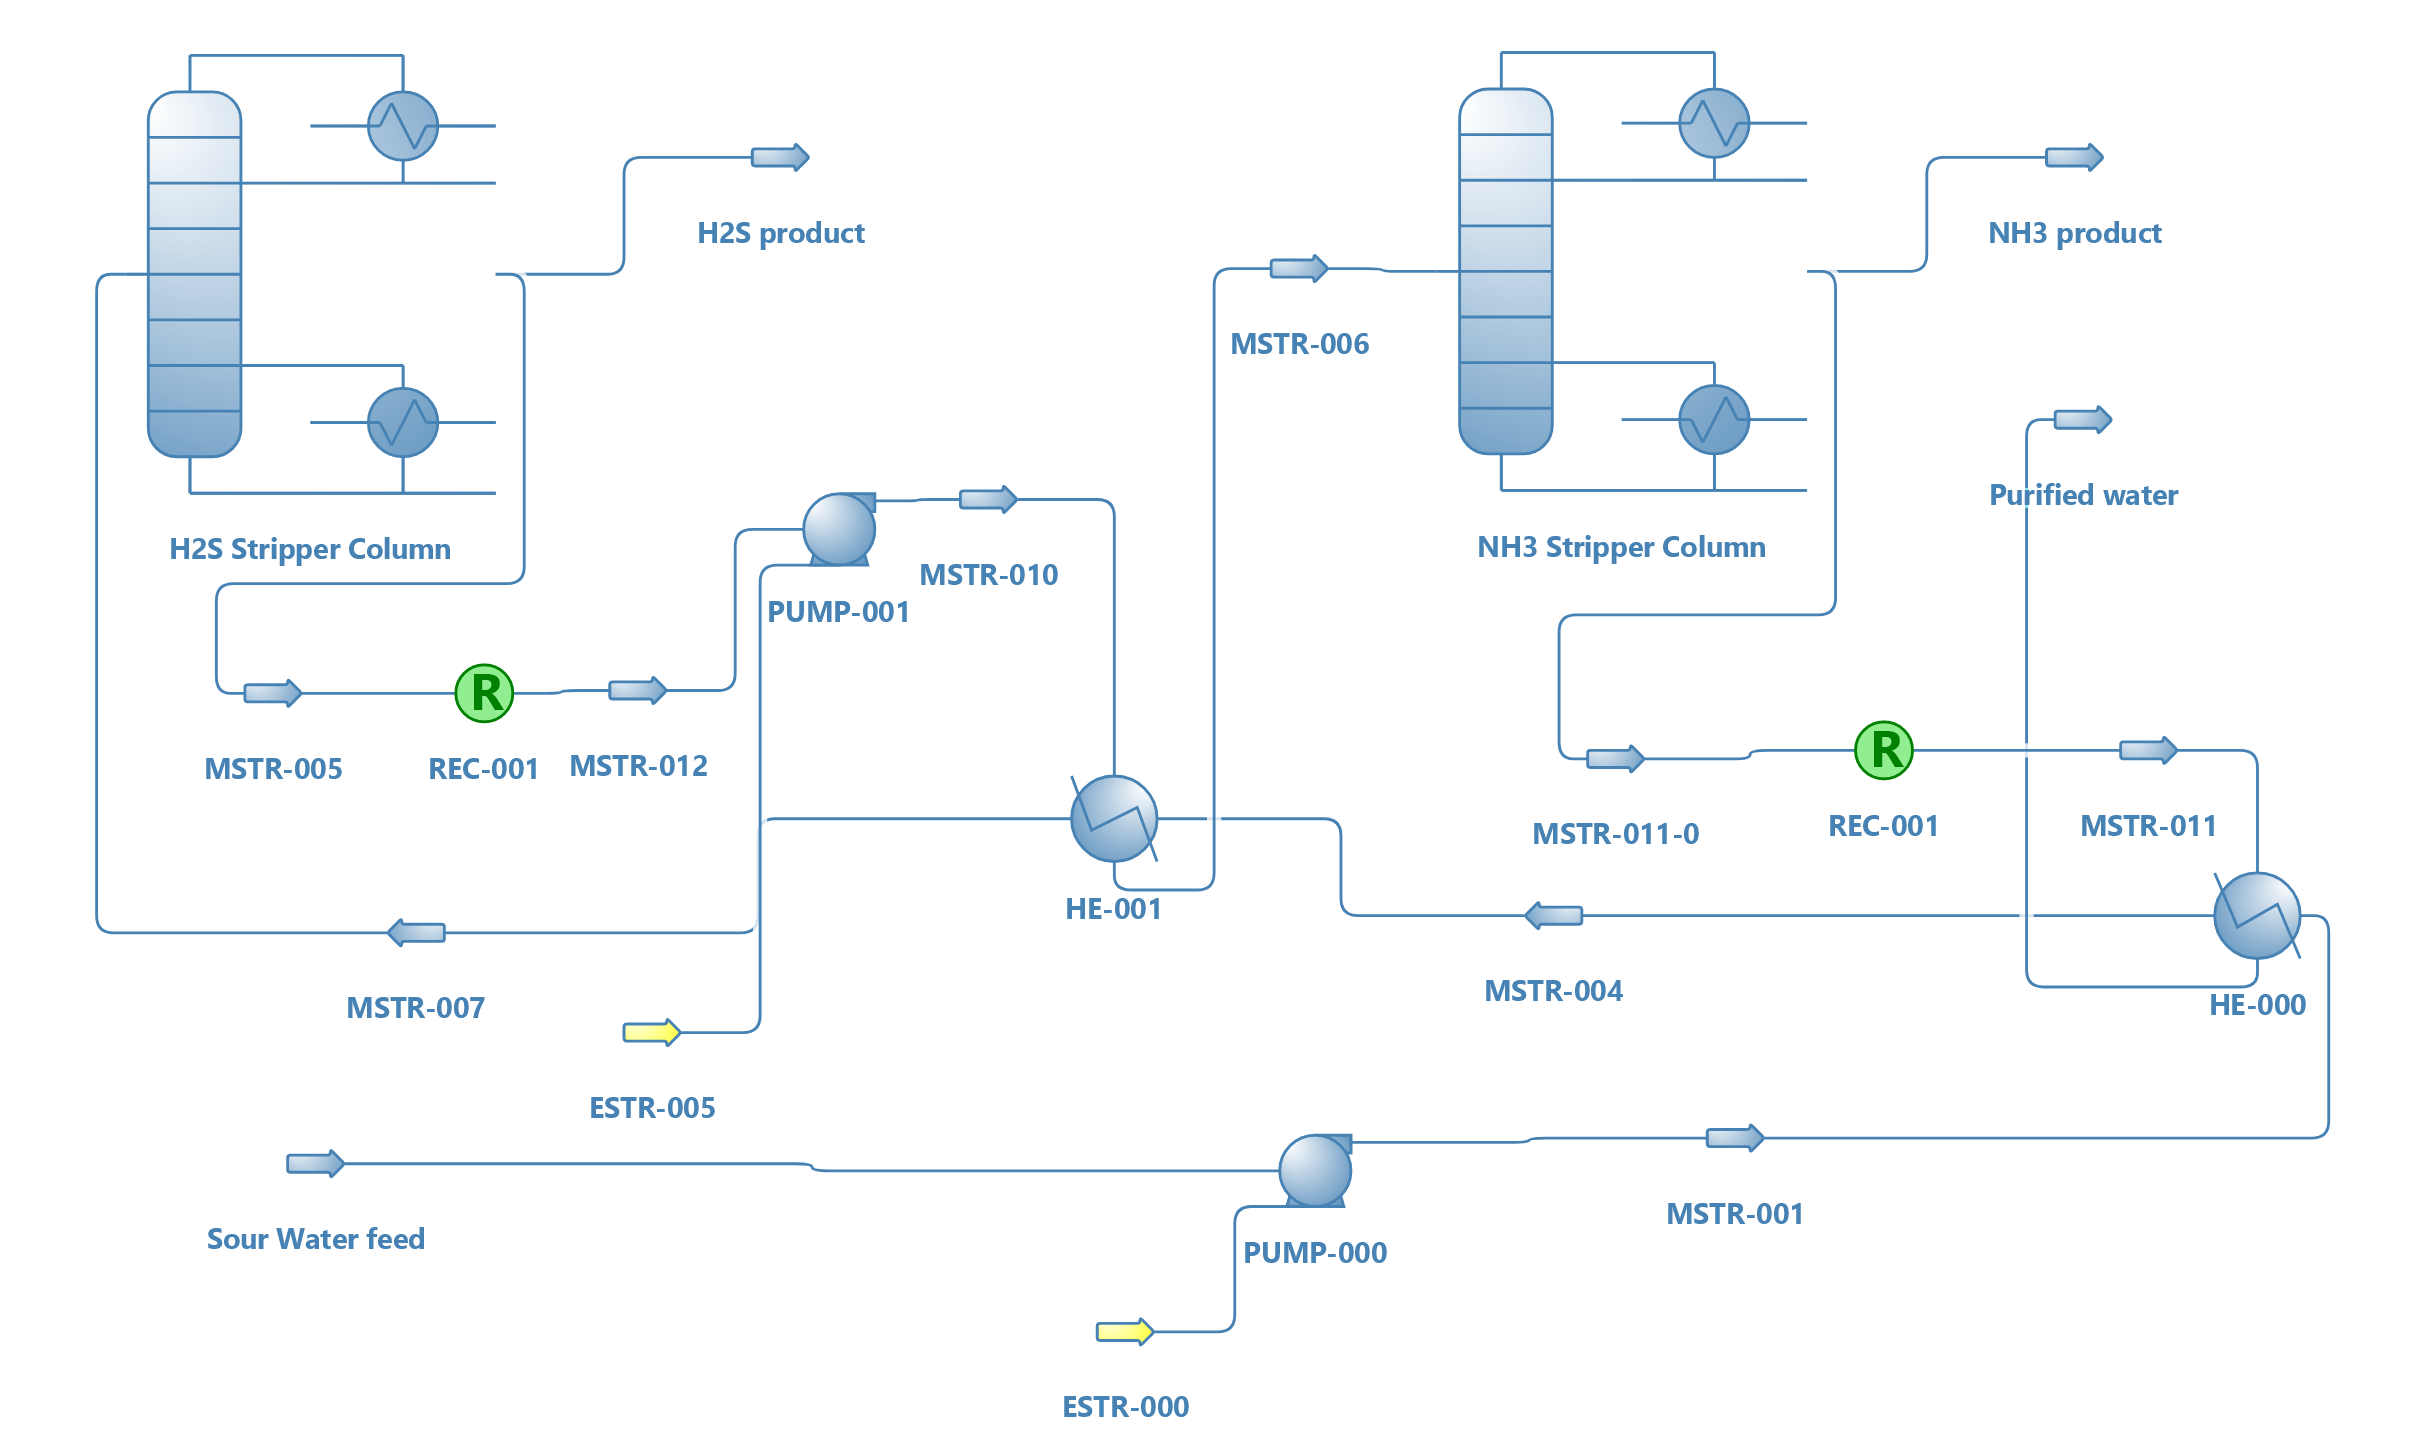
\includegraphics[width=0.85\linewidth]{Sour-Water.png}}

\newpage
\noindent \textbf{Results:}
\begin{table}[ht]
\centering
\resizebox{\textwidth}{!}{%
\begin{tabular}{|l|l|l|l|l|l|}
\hline
Object                                   & NaOH + EtOH & NaOH + EtOH + Oil & Reaction Products (M1) & M1**     &       \\ \hline
Temperature                              & 25.06392    & 51.07824          & 51.20892               & 44.67    & C     \\ \hline
Pressure                                 & 1           & 1                 & 1                      & 0.296077 & atm   \\ \hline
Mass Flow                                & 79.030073   & 303.2891          & 303.2891               & 303.2891 & g/s   \\ \hline
Molar Flow                               & 1.722756    & 2.000534          & 2.000539               & 2.000539 & mol/s \\ \hline
Mass Fraction (Mixture)  /  Ethanol\_BD  & 0.971569    & 0.253168          & 0.132914               & 0.132914 &       \\ \hline
Mass Fraction (Mixture)  /  EtP          & 0.000031    & 0.000008          & 0.742583               & 0.742583 &       \\ \hline
Mass Fraction (Mixture)  /  PPP          & 0           & 0.739423          & 0.036971               & 0.036971 &       \\ \hline
Mass Fraction (Mixture)  /  NaOH\_BD     & 0.028369    & 0.007392          & 0.007392               & 0.007392 &       \\ \hline
Mass Fraction (Mixture)  /  Glycerol\_BD & 0.000031    & 0.000008          & 0.080139               & 0.080139 &       \\ \hline
\end{tabular}%
}
\end{table}
\begin{table}[ht]
\centering
\resizebox{\textwidth}{!}{%
\begin{tabular}{|l|l|l|l|l|l|l|}
\hline
Object                                   & M1**       & Biodiesel + Impurities & Bottoms (Biodiesel) & Water + Impurities & Biodiesel Product &       \\ \hline
Temperature                              & 44.67      & 214.6771               & 60.00389            & 147.0185           & 25                & C     \\ \hline
Pressure                                 & 0.296077   & 0.296077               & 1                   & 1                  & 1                 & atm   \\ \hline
Mass Flow                                & 303.289073 & 263.5016               & 224.3065            & 305.2663           & 224.3065          & g/s   \\ \hline
Molar Flow                               & 2.000539   & 1.136907               & 0.781696            & 15.12477           & 0.781696          & mol/s \\ \hline
Mass Fraction (Mixture)  /  Ethanol\_BD  & 0.132914   & 0.001988               & 0.000519            & 0.001334           & 0.000519          &       \\ \hline
Mass Fraction (Mixture)  /  Water\_BD    & 0          & 0.09224                & 0                   & 0.871618           & 0                 &       \\ \hline
Mass Fraction (Mixture)  /  Glycerol\_BD & 0.080139   & 0.85471                & 0                   & 0.079613           & 0                 &       \\ \hline
Mass Fraction (Mixture)  /  EtP          & 0.742583   & 0.008509               & 0.982058            & 0.016165           & 0.982058          &       \\ \hline
Mass Fraction (Mixture)  /  NaOH\_BD     & 0.007392   & 0.042554               & 0                   & 0.007343           & 0                 &       \\ \hline
Mass Fraction (Mixture)  /  PPP          & 0.036971   & 0.042554               & 0.017423            & 0.023926           & 0.017423          &       \\ \hline
\end{tabular}%
}
\caption{Streamwise Results for Biodiesel Production}
\end{table}

\end{document}


